% TiKz
\documentclass[tikz, 12pt]{standalone}
\usetikzlibrary{positioning}
\usetikzlibrary{shapes}

% Math
\usepackage{amsfonts}
\usepackage{amsmath}

% CMU sans serif font.
\usepackage[T1]{fontenc}
\renewcommand*\familydefault{\sfdefault}

\begin{document}
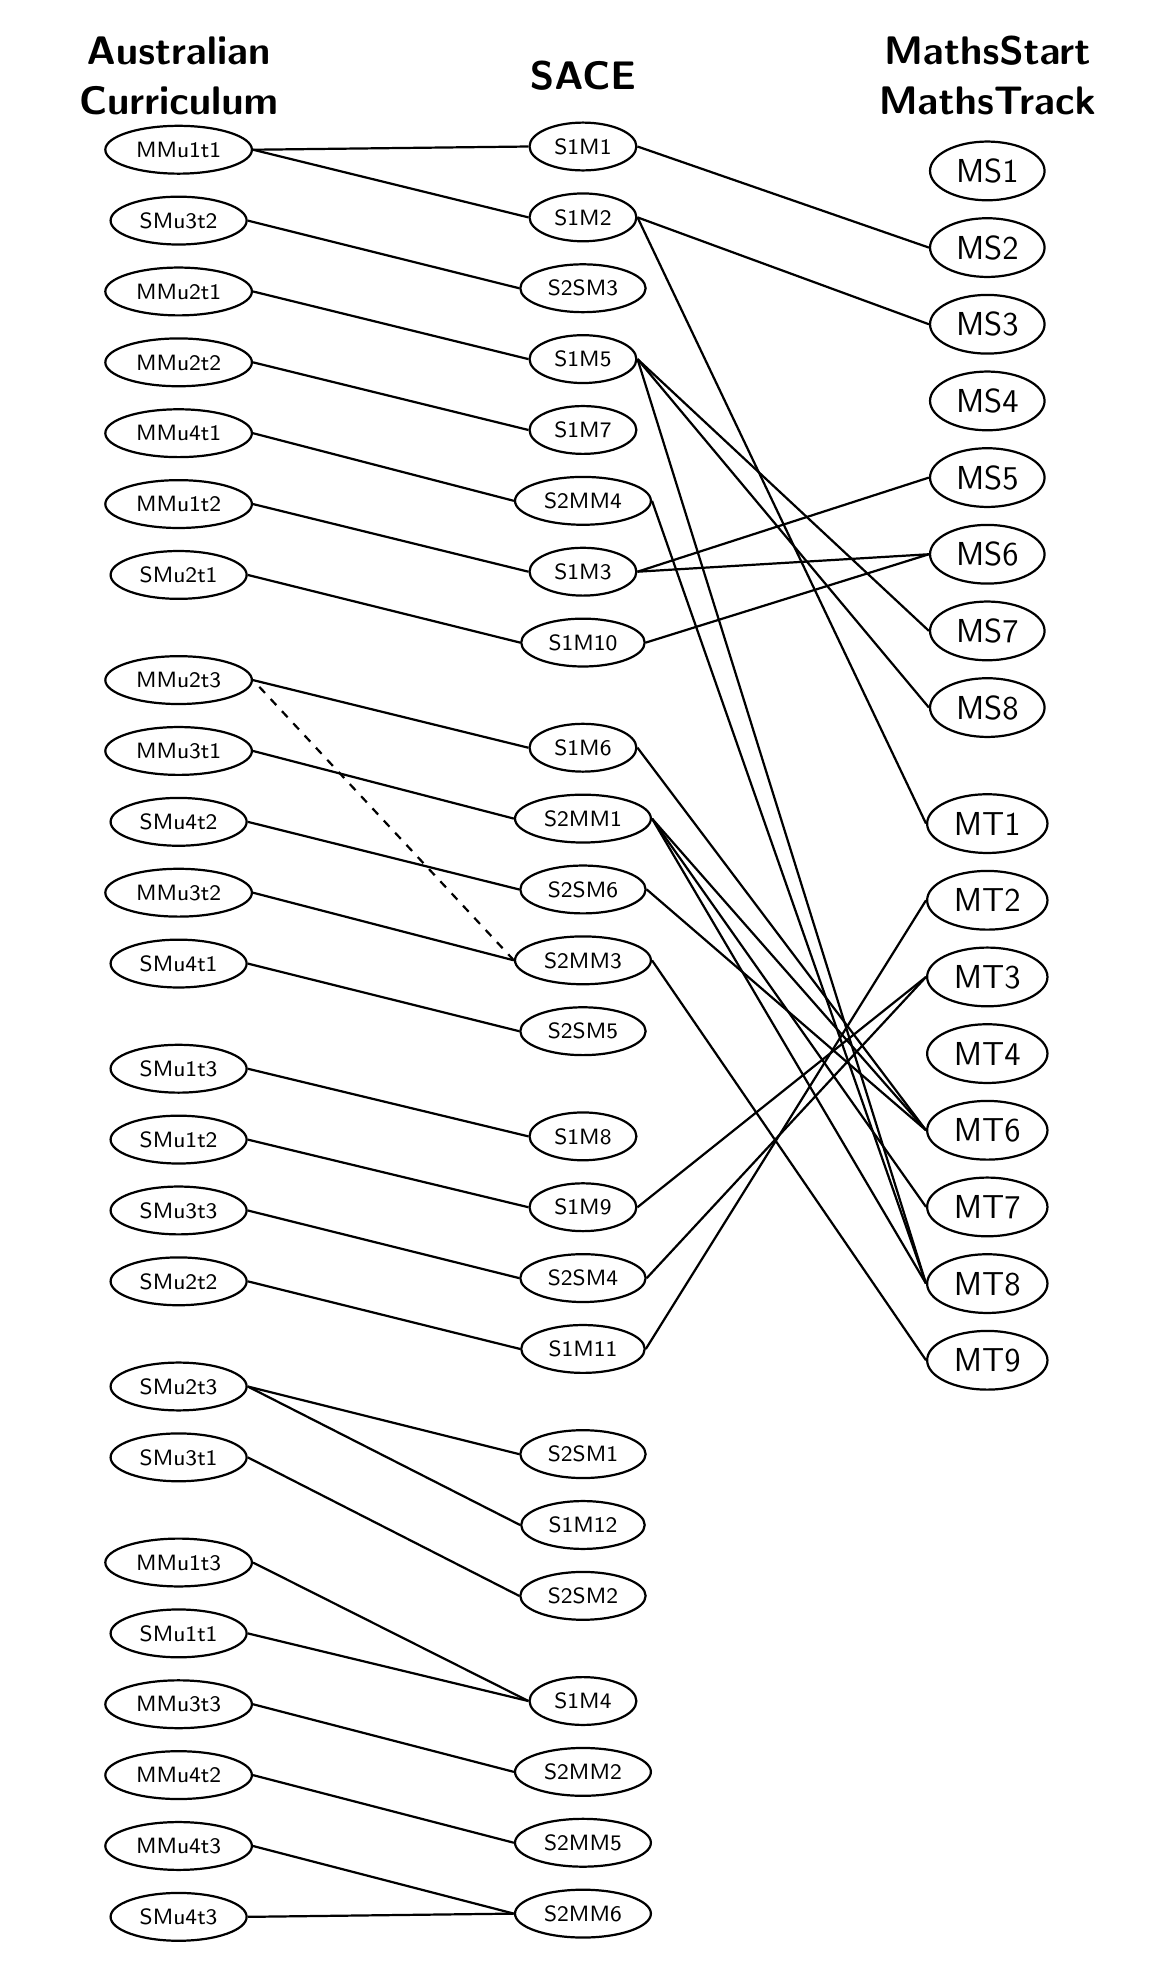
\begin{tikzpicture}[node distance=0.9cm,thick,topic node/.style={ellipse,draw,font=\footnotesize},unit node/.style={ellipse,draw,font=\large}]

	% MathsStart
	\node[font=\Large\bfseries, text width = 3.6cm, align=center] (ms) {MathsStart MathsTrack};
  	\node[unit node] (ms1) [below=0.2cm of ms] {MS1};
  	\node[unit node] (ms2) [below=0.2cm of ms1] {MS2};
  	\node[unit node] (ms3) [below=0.2cm of ms2] {MS3};
  	\node[unit node] (ms4) [below=0.2cm of ms3] {MS4};
  	\node[unit node] (ms5) [below=0.2cm of ms4] {MS5};
  	\node[unit node] (ms6) [below=0.2cm of ms5] {MS6};
  	\node[unit node] (ms7) [below=0.2cm of ms6] {MS7};
  	\node[unit node] (ms8) [below=0.2cm of ms7] {MS8};
%  	\node[unit node] (ms1) [below=0.2cm of ms] {Functions};
%  	\node[unit node] (ms2) [below=0.2cm of ms1] {Linear};
%  	\node[unit node] (ms3) [below=0.2cm of ms2] {Quadratic};
%  	\node[unit node] (ms4) [below=0.2cm of ms3] {Rational};
%  	\node[unit node] (ms5) [below=0.2cm of ms4] {Trigonometry I};
%  	\node[unit node] (ms6) [below=0.2cm of ms5] {Trigonometry II};
%  	\node[unit node] (ms7) [below=0.2cm of ms6] {Exponential};
%  	\node[unit node] (ms8) [below=0.2cm of ms7] {Logarithm};

	% MathsTrack
  	\node[unit node] (mt1) [below=0.7cm of ms8] {MT1};
  	\node[unit node] (mt2) [below=0.2cm of mt1] {MT2};
  	\node[unit node] (mt3) [below=0.2cm of mt2] {MT3};
  	\node[unit node] (mt4) [below=0.2cm of mt3] {MT4};
  	\node[unit node] (mt6) [below=0.2cm of mt4] {MT6};
  	\node[unit node] (mt7) [below=0.2cm of mt6] {MT7};
  	\node[unit node] (mt8) [below=0.2cm of mt7] {MT8};
  	\node[unit node] (mt9) [below=0.2cm of mt8] {MT9};
%  	\node[unit node] (mt1) [below=0.8cm of ms8] {Polynomials};
%  	\node[unit node] (mt2) [below=0.2cm of mt1] {Matrices};
%  	\node[unit node] (mt3) [below=0.2cm of mt2] {Vectors};
%  	\node[unit node] (mt4) [below=0.2cm of mt3] {Systems of Eqns};
%  	\node[unit node] (mt6) [below=0.2cm of mt4] {Differentiation};
%  	\node[unit node] (mt7) [below=0.2cm of mt6] {Differentiation Apps};
%  	\node[unit node] (mt8) [below=0.2cm of mt7] {Exp and Log};
%  	\node[unit node] (mt9) [below=0.2cm of mt8] {Integration};
  	
	% SACE
	\node[font=\Large\bfseries] (sace) [left=2.4cm of ms] {SACE};
	% Functions and Graphs
  	\node[topic node] (ss1m1) [below of=sace] {S1M1};
  	\node[topic node] (ss1m2) [below of=ss1m1] {S1M2};
  	\node[topic node] (ss2sm3) [below of=ss1m2] {S2SM3};
  	\node[topic node] (ss1m5) [below of=ss2sm3] {S1M5};
  	\node[topic node] (ss1m7) [below of=ss1m5] {S1M7};
  	\node[topic node] (ss2mm4) [below of=ss1m7] {S2MM4};
  	\node[topic node] (ss1m3) [below of=ss2mm4] {S1M3};
  	\node[topic node] (ss1m10) [below of=ss1m3] {S1M10};
	% Calculus
  	\node[topic node] (ss1m6) [below=0.7cm of ss1m10] {S1M6};
  	\node[topic node] (ss2mm1) [below of=ss1m6] {S2MM1};
  	\node[topic node] (ss2sm6) [below of=ss2mm1] {S2SM6};  	
  	\node[topic node] (ss2mm3) [below of=ss2sm6] {S2MM3};
  	\node[topic node] (ss2sm5) [below of=ss2mm3] {S2SM5};
	% Geometry and Linear Algebra
  	\node[topic node] (ss1m8) [below=0.7cm of ss2sm5] {S1M8};
	\node[topic node] (ss1m9) [below of=ss1m8] {S1M9};
  	\node[topic node] (ss2sm4) [below of=ss1m9] {S2SM4};
  	\node[topic node] (ss1m11) [below of=ss2sm4] {S1M11};
  	% Complex Numbers
  	\node[topic node] (ss2sm1) [below=0.7cm of ss1m11] {S2SM1};
  	\node[topic node] (ss1m12) [below of=ss2sm1] {S1M12};
  	\node[topic node] (ss2sm2) [below of=ss1m12] {S2SM2};
	% Probability and Statistics	
  	\node[topic node] (ss1m4) [below=0.7cm of ss2sm2] {S1M4};
  	\node[topic node] (ss2mm2) [below of=ss1m4] {S2MM2}; 	
  	\node[topic node] (ss2mm5) [below of=ss2mm2] {S2MM5};
  	\node[topic node] (ss2mm6) [below of=ss2mm5] {S2MM6};
  	
  	
	% Australian Curriculum
	\node[font=\Large\bfseries, text width = 3.6cm, align=center] (ac) [left=2.4cm of sace] {Australian Curriculum};
	% Functions and Graphs
  	\node[topic node] (acmmmu1t1) [below=0cm of ac] {MMu1t1};
  	\node[topic node] (acmsmu3t2) [below of=acmmmu1t1] {SMu3t2};
  	\node[topic node] (acmmmu2t1) [below of=acmsmu3t2] {MMu2t1};
  	\node[topic node] (acmmmu2t2) [below of=acmmmu2t1] {MMu2t2};
  	\node[topic node] (acmmmu4t1) [below of=acmmmu2t2] {MMu4t1};
  	\node[topic node] (acmmmu1t2) [below of=acmmmu4t1] {MMu1t2};
  	\node[topic node] (acmsmu2t1) [below of=acmmmu1t2] {SMu2t1};
	% Calculus
  	\node[topic node] (acmmmu2t3) [below=0.7cm of acmsmu2t1] {MMu2t3};
  	\node[topic node] (acmmmu3t1) [below of=acmmmu2t3] {MMu3t1};
  	\node[topic node] (acmsmu4t2) [below of=acmmmu3t1] {SMu4t2};
  	\node[topic node] (acmmmu3t2) [below of=acmsmu4t2] {MMu3t2};
  	\node[topic node] (acmsmu4t1) [below of=acmmmu3t2] {SMu4t1};
	% Geometry and Linear Algebra
  	\node[topic node] (acmsmu1t3) [below=0.7cm of acmsmu4t1] {SMu1t3};
  	\node[topic node] (acmsmu1t2) [below of=acmsmu1t3] {SMu1t2};
  	\node[topic node] (acmsmu3t3) [below of=acmsmu1t2] {SMu3t3};
  	\node[topic node] (acmsmu2t2) [below of=acmsmu3t3] {SMu2t2};
	% Complex Numbers
  	\node[topic node] (acmsmu2t3) [below=0.7cm of acmsmu2t2] {SMu2t3};
  	\node[topic node] (acmsmu3t1) [below of=acmsmu2t3] {SMu3t1};
	% Probability and Statistics
  	\node[topic node] (acmmmu1t3) [below=0.7cm of acmsmu3t1] {MMu1t3};
  	\node[topic node] (acmsmu1t1) [below of=acmmmu1t3] {SMu1t1};
  	\node[topic node] (acmmmu3t3) [below of=acmsmu1t1] {MMu3t3};
  	\node[topic node] (acmmmu4t2) [below of=acmmmu3t3] {MMu4t2};
  	\node[topic node] (acmmmu4t3) [below of=acmmmu4t2] {MMu4t3};
  	\node[topic node] (acmsmu4t3) [below of=acmmmu4t3] {SMu4t3};

	% Australian Curriculum -- SACE links
	\draw (ss1m1.west) -- (acmmmu1t1.east);
	\draw (ss1m2.west) -- (acmmmu1t1.east);
	\draw (ss1m3.west) -- (acmmmu1t2.east);
	\draw (ss1m4.west) -- (acmmmu1t3.east);
	\draw (ss1m4.west) -- (acmsmu1t1.east);
	\draw (ss1m5.west) -- (acmmmu2t1.east);
	\draw (ss1m6.west) -- (acmmmu2t3.east);
	\draw (ss1m7.west) -- (acmmmu2t2.east);
	\draw (ss1m8.west) -- (acmsmu1t3.east);
	\draw (ss1m9.west) -- (acmsmu1t2.east);
	\draw (ss1m10.west) -- (acmsmu2t1.east);
	\draw (ss1m11.west) -- (acmsmu2t2.east);
	\draw (ss1m12.west) -- (acmsmu2t3.east);
		
	\draw (ss2mm1.west) -- (acmmmu3t1.east);
	\draw (ss2mm2.west) -- (acmmmu3t3.east);
	\draw (ss2mm3.west) -- (acmmmu3t2.east);
	\draw[dashed] (ss2mm3.west) -- (acmmmu2t3.east);
	\draw (ss2mm4.west) -- (acmmmu4t1.east);
	\draw (ss2mm5.west) -- (acmmmu4t2.east);
	\draw (ss2mm6.west) -- (acmmmu4t3.east);
	\draw (ss2mm6.west) -- (acmsmu4t3.east);

	\draw (ss2sm1.west) -- (acmsmu2t3.east);
	\draw (ss2sm2.west) -- (acmsmu3t1.east);
	\draw (ss2sm3.west) -- (acmsmu3t2.east);
	\draw (ss2sm4.west) -- (acmsmu3t3.east);
	\draw (ss2sm5.west) -- (acmsmu4t1.east);
	\draw (ss2sm6.west) -- (acmsmu4t2.east);

	% MathsTrack to SACE links
	\draw (mt1.west) -- (ss1m2.east);
	\draw (mt2.west) -- (ss1m11.east);
	\draw (mt3.west) -- (ss1m9.east);
	\draw (mt3.west) -- (ss2sm4.east);
	\draw (mt6.west) -- (ss1m6.east);
	\draw (mt6.west) -- (ss2mm1.east);
	\draw (mt6.west) -- (ss2sm6.east);
	\draw (mt7.west) -- (ss2mm1.east);
	\draw (mt8.west) -- (ss1m5.east);
	\draw (mt8.west) -- (ss2mm1.east);
	\draw (mt8.west) -- (ss2mm4.east);
	\draw (mt9.west) -- (ss2mm3.east);

	% MathsTrack to SACE links
	\draw (ms2.west) -- (ss1m1.east);
	\draw (ms3.west) -- (ss1m2.east);
	\draw (ms5.west) -- (ss1m3.east);
	\draw (ms6.west) -- (ss1m3.east);
	\draw (ms6.west) -- (ss1m10.east);
	\draw (ms7.west) -- (ss1m5.east);
	\draw (ms8.west) -- (ss1m5.east);


  	
\end{tikzpicture}
\end{document}